\documentclass{article}
% --- General Packages ---
\usepackage[utf8]{inputenc}
\usepackage[T1]{fontenc}
\usepackage[english]{babel}
\usepackage{fullpage}
\usepackage{geometry}
\usepackage{graphicx}
\usepackage{hyperref}
\usepackage{url}
\usepackage{setspace}
\usepackage{comment}
\usepackage{xcolor}

% --- Math Packages ---
\usepackage{amsmath,amssymb,amsthm,nccmath}
\usepackage{amsfonts}
\usepackage{bm}

% --- Table & Figure Packages ---
\usepackage{booktabs}
\usepackage{multirow}
\usepackage{float}

% --- Code & Text Packages ---
\usepackage{listings}
\usepackage[autostyle, english = american]{csquotes}
\usepackage{algpseudocode}
\usepackage{tikz}
\usepackage{subcaption}
\usetikzlibrary {automata,positioning}

% --- Listing Style Configuration ---
\definecolor{codegreen}{rgb}{0,0.6,0}
\definecolor{codegray}{rgb}{0.5,0.5,0.5}
\definecolor{codepurple}{rgb}{0.58,0,0.82}
\definecolor{backcolour}{rgb}{0.95,0.95,0.92}

\lstdefinestyle{mystyle}{
    backgroundcolor=\color{backcolour},
    commentstyle=\color{codegreen},
    keywordstyle=\color{magenta},
    numberstyle=\tiny\color{codegray},
    stringstyle=\color{codepurple},
    basicstyle=\ttfamily\scriptsize,
    breakatwhitespace=false,
    breaklines=true,
    captionpos=b,
    keepspaces=true,
    numbers=left,
    numbersep=1pt,
    showspaces=false,
    showstringspaces=false,
    showtabs=false,
    tabsize=2,
    inputencoding=utf8,
    extendedchars=true,
}
\lstset{style=mystyle,
    literate={«}{{\guillemotleft}}1{»}{{\guillemotright}}1{’}{{\textquoteright}}1
}
\setlength{\parindent}{0in}
\setlength{\parindent}{0in}
\begin{document}
\begin{titlepage}
	\begin{center}
		\vspace*{1cm}

		\Huge
		\textbf{Devoir 2}

		\vspace{0.5cm}
		\LARGE

		\vspace{1.5cm}

        
		\textbf{Samuel Fournier}\\20218212 \\
		\vfill
		\textbf{Alexandre Toutant}\\20028191 \\
		\vfill


		Dans le cadre du cours\\
		IFT 6150


		\vspace{0.8cm}

		
\includegraphics[width=0.4\textwidth]{udem.jpg}

		\Large
		Département d'informatique et de recherche opérationnelle\\
		Université de Montréal\\
		Canada\\
		29 octobre 2025

	\end{center}
\end{titlepage}
\section*{Introduction}

Ce travail pratique avait pour but de programmer, en langage C, les principales étapes du détecteur de contours de \textbf{Canny}.  
L'objectif était de comprendre comment on peut passer d'une image en niveaux de gris à une image contenant seulement les contours importants, tout en réduisant le bruit et les faux contours.

\subsection*{But du TP}
Le but du TP était de réaliser un programme capable de détecter les contours d’une image.  
Pour y arriver, le programme effectue les étapes suivantes :
\begin{enumerate}
    \item Appliquer un \textbf{flou gaussien} pour réduire le bruit;
    \item Calculer le \textbf{gradient} d’intensité avec les filtres \((-1,1)\);
    \item Trouver la \textbf{direction du gradient} (0°, 45°, 90°, 135°);
    \item Faire la \textbf{suppression des non-maximums} pour amincir les contours;
    \item Appliquer un \textbf{double seuillage} (\(\tau_L\), \(\tau_H\)) avec un suivi par hystérésis pour ne garder que les vrais bords.
\end{enumerate}

\subsection*{Rôle des contours}
Les contours représentent les zones où l’intensité change brusquement.  
Ils délimitent les objets et aident à comprendre la structure d’une image.  
La détection de contours est essentielle pour plusieurs applications : segmentation d’objets, reconnaissance de formes, suivi de mouvement, etc.  
Un bon détecteur doit être à la fois précis, résistant au bruit et produire des bords fins et continus.

\subsection*{Filtre gaussien}
Avant la détection des contours, un \textbf{filtre gaussien} est appliqué pour adoucir l’image et éliminer le bruit.  
Cela empêche le détecteur de confondre les petites variations d’intensité avec de faux contours.  
Dans notre code, ce filtrage est effectué dans le \textbf{domaine fréquentiel} à l’aide de la \textbf{transformée de Fourier (FFT)}.  
Le paramètre \(\sigma\) contrôle l’intensité du flou :
\begin{itemize}
    \item petit \(\sigma\) : plus de détails visibles;
    \item grand \(\sigma\) : image plus lissée, moins de bruit.
\end{itemize}
Cette étape prépare l’image pour le calcul du gradient et assure une détection de contours plus stable.
Voici le résultat du filtre sur l'image avec quelques valeurs de $\sigma$ différentes:
\begin{figure}[H]
    \centering
    \begin{subfigure}[b]{0.45\linewidth}
        \centering
        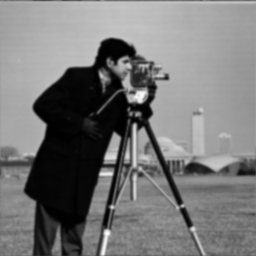
\includegraphics[scale = 0.5]{TpIFT6150-2-filtre-gaussien_1.png}
        \caption{Filtre gaussien avec $\sigma = 1$}
    \end{subfigure}
    \begin{subfigure}[b]{0.45\linewidth}
        \centering
        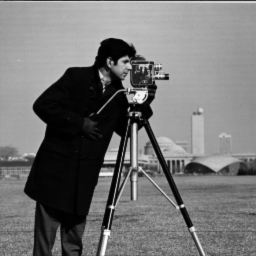
\includegraphics[scale = 0.5]{TpIFT6150-2-filtre-gaussien_05.png}
        \caption{Filtre gaussien avec $\sigma = 0.5$}
    \end{subfigure}
    \vspace{1em}
    \begin{subfigure}[b]{0.45\linewidth}
        \centering
        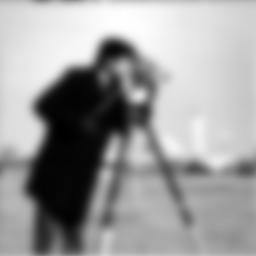
\includegraphics[scale = 0.5]{TpIFT6150-2-filtre-gaussien_5.png}
        \caption{Filtre gaussien avec $\sigma = 5$}
    \end{subfigure}
    \begin{subfigure}[b]{0.45\linewidth}
        \centering
        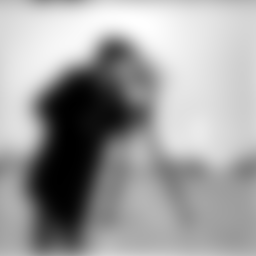
\includegraphics[scale = 0.5]{TpIFT6150-2-filtre-gaussien_10.png}
        \caption{Filtre gaussien avec $\sigma = 10$}
    \end{subfigure}
    \caption{Différents résultats de \textit{blurring}}
\end{figure}

\section*{Description de la méthode utilisée pour calculer le gradient, la norme et l'angle}

Le calcul du gradient permet d’identifier les zones de l’image où l’intensité varie le plus rapidement, ce qui correspond aux contours.  
Dans notre programme, le gradient est obtenu à l’aide des filtres de convolution \([-1, 1]\), appliqués séparément sur les directions horizontales et verticales.

\subsection*{Calcul du gradient}
Pour chaque pixel, deux dérivées sont calculées :
\begin{itemize}
    \item \( G_x = I(x, y+1) - I(x, y) \) pour la variation horizontale;
    \item \( G_y = I(x+1, y) - I(x, y) \) pour la variation verticale.
\end{itemize}
Ces filtres simples permettent d’estimer la direction et l’intensité du changement local dans l’image.

\subsection*{Norme du gradient}
La norme du gradient indique l'intensité du contour à chaque point :
\[
G = \sqrt{G_x^2 + G_y^2}
\]
Plus la norme est grande, plus le contour est fort.  
C’est cette valeur qui est utilisée plus tard pour la suppression des non-maximums et pour l’hystérésis.
Voici de quoi l'image à l'air lorsque l'on visualize les normes des gradients:
\begin{figure}[H]
    \centering
    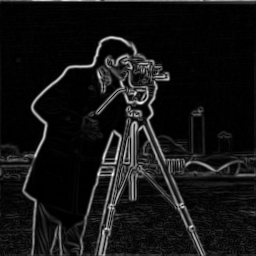
\includegraphics[scale = 0.5]{TpIFT6150-2-gradient.png}
    \caption{Normes des gradients avec $\sigma = 1$}
\end{figure}

\subsection*{Angle du gradient}
L’orientation du gradient est donnée par :
\[
\theta = \arctan{\left(\frac{G_y}{G_x}\right)}
\]
Dans le programme, cet angle est converti en degrés et ramené dans l’intervalle \([0,180]\).  
Il est ensuite estimé selon quatre directions principales : 0°, 45°, 90° et 135°, ce qui simplifie la comparaison des pixels lors de la suppression des non-maximums.

\section*{Dénombrer le nombre de seuils dans le filtre de Canny}

Le filtre de Canny utilise \textbf{deux seuils} : un seuil bas (\(\tau_L\)) et un seuil haut (\(\tau_H\)).  
Le seuil haut sert à détecter les contours forts, tandis que le seuil bas garde les contours plus faibles s’ils sont reliés à un contour fort.  
Les pixels sous \(\tau_L\) sont ignorés.  
Ce double seuillage permet de conserver des bords continus tout en réduisant les faux contours causés par le bruit.

\section*{Description de la méthode utilisée pour calculer les seuils à partir de l'histogramme}
\subsection*{Méthode sans \textbf{bin}}
La méthode utilisée est une méthode d'histogramme simple. Juste avant la supression des non-maximums, on créé une liste de longueur $length \times width$ qui contient tous
les gradients de tous les pixels:
\begin{lstlisting}[language=c]
    float* sortedGrads = fmatrix_allocate_1d(height * width);
\end{lstlisting}
Ensuite, on utilise un algorithme de trie très rudimentaire (et lent) pour trier les valeurs des gradient dans cette liste:
\begin{lstlisting}[language=C]
void sortList(float* list, int size) {
    float key;
    int j;

    for (int i = 1; i < size; i++) {
        key = list[i]; // Store the current element to be inserted
        j = i - 1;

        // Move elements of sortedGrads[0..i-1] that are greater than key
        // to one position ahead of their current position
        while (j >= 0 && list[j] > key) {
            list[j + 1] = list[j];
            j = j - 1;
        }
        list[j + 1] = key; // Insert the key into its correct spot
    }
}
\end{lstlisting}
Une fois la liste triée, on utilise la valeur de la variable $p\_H$ pour déterminer la valeur de $\tau_h$ et de $\tau_l$. Pour trouver la valeur de $\tau_h$ 
choisit le gradient se trouvant au $p\_H$ ième percentile de la liste. Par exemple, si on a que $p\_H = 0.9$, on choisit la valeur du gradient se trouvant à 
l'index qui se trouve à $90\%$ de la liste.
\begin{lstlisting}[language=C]
    int indexToCut = (int)floor((float)(length * width) * p_H);
    float tau_h = sortedGrads[indexToCut];
\end{lstlisting}
Finalement, pour obtenir $\tau_l$, on multiplie $\tau_h$ par $0.5$.
\begin{lstlisting}[language=C]
    float tau_l = 0.5 * tau_h;
\end{lstlisting}
Une fois les valeurs de $\tau_h$ et $\tau_l$ calculer, on continue l'algorithme comme normale en faisant la supression des non-maximums
et du seuillage par hystérisis. \\\\
Avec une valeur de $p_H$ de $0.9$, on obtient $\tau_h = 65.23$ et $\tau_l = 32.62$ (deux valeurs très proche du 66 et 33 utilisé lors de l'ancienne méthode). 
Avec ces valeurs, on obtient l'image suivante:
\begin{figure}[H]
    \center
    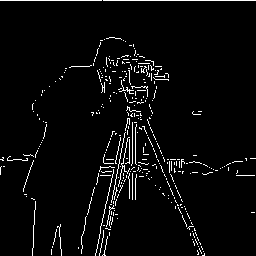
\includegraphics[scale=0.5]{TpIFT6150-2-canny_09.png}
    \caption{Résultat final avec $\sigma = 1$ et $p_H = 0.9$}
\end{figure}
Si on diminue la valeur de $p_H$ à 0.7, on observe que l'algorithme préserve beaucoup plus de contours qu'avant:
\begin{figure}[H]
    \center
    
\includegraphics[scale=0.5]{TpIFT6150-2-canny_07.png}
    \caption{Résultat final avec $\sigma = 1$ et $p_H = 0.7$}
\end{figure}
Finalement avec une valeur de $p_H$ de $0.95$, on voit qu'il y a moins de contours de préservés:
\begin{figure}[H]
    \center
    
\includegraphics[scale=0.5]{TpIFT6150-2-canny_095.png}
    \caption{Résultat final avec $\sigma = 1$ et $p_H = 0.95$}
\end{figure}
\subsection*{Méthode avec \textbf{bin}}
La grande différence entre cette méthode et la méthode précédente est comment on choisit la valeur pour $\tau_H$. Plutôt que de trier une liste
contenant tous les gradients et sélectionner le gradient au $p_H$ième percentile, on place tous les gradients dans des \textbf{bins} basé sur la valeur
de leur norme. Par exemple, on pourrait avoir 100 \textbf{bins} avec un intervalle de valeurs de 10, ce qui voudrait dire que tous les gradients ayant une norme
entre 0 et 10 irait dans le \textbf{bin} 0, etc... 
\begin{lstlisting}[language=C]
float bin_width = g_max / (float)NUM_BINS;
    
// 1. Initialize Histogram Bins (Array of structs)
Bin histogram[NUM_BINS];
for (int i = 0; i < NUM_BINS; ++i) {
    histogram[i].sum = 0.0f;
    histogram[i].count = 0;
    // Allocate initial memory for the content (will be reallocated later)
    histogram[i].capacity = MAX_BIN_CAPACITY;
    histogram[i].content = (float*)malloc(sizeof(float) * MAX_BIN_CAPACITY);
    if (histogram[i].content == NULL) {
        return;
    }
}
// 2. Populate Bucketint bin_index
for (int i = 0; i < height; ++i) {
    for (int j = 0; j < width; ++j) {
        float g = norms[i][j];
            
        // Calculate bin index (clamp to last bin if exactly g_max)
        bin_index = (int)floorf(g / bin_width);
        if (bin_index >= NUM_BINS) {
            bin_index = NUM_BINS - 1; 
        }
            
        // Check if capacity needs to be increased (dynamic list)
        if (histogram[bin_index].count >= histogram[bin_index].capacity) {
            histogram[bin_index].capacity *= 2;
            histogram[bin_index].content = (float*)realloc(histogram[bin_index].content, 
                                        sizeof(float) * histogram[bin_index].capacity);
            if (histogram[bin_index].content == NULL) {
                return;
            }
        }
            

        // Store gradient, update sum and count
        histogram[bin_index].content[histogram[bin_index].count] = g;
        histogram[bin_index].sum += g;
        histogram[bin_index].count++;
    }
}

// 3. Find the Percentile Bin and Calculate tau_H
int total_pixels = height * width;
int target_count = (int)floorf((float)total_pixels * pH);
int cumulative_count = 0;
int percentile_bin_index = -1;

for (int i = 0; i < NUM_BINS; ++i) {
    cumulative_count += histogram[i].count;
    if (cumulative_count >= target_count) {
        percentile_bin_index = i;
        break;
    }
}
\end{lstlisting}
Une fois tous les gradients placés dans leur \textbf{bin} respectif, on détermine quel bin contient
le gradient se trouvant au $p_H$ième percentile. Une fois que cela soit fait, on peut procéder de deux façons différentes. Soit que $\tau_H = avg(bin)$ ou 
$\tau_H = median(bin)$. Dans les deux cas, les valeurs de $\tau_H$ et $\tau_L$ sont très proches à celles de la première méthode, alors les résultats sont 
essentiellements les mêmes.


\section*{Description de l’approximation de l’angle}

L’angle du gradient est calculé à l’aide de la fonction \(\arctan\left(\frac{G_y}{G_x}\right)\), ce qui donne une valeur comprise entre \(0\) et \(180\) degrés.  
Pour simplifier le traitement lors de la suppression des non-maximums, on ne garde pas l’angle exact.  
On retourne plutôt la valeur parmi \(0^\circ\), \(45^\circ\), \(90^\circ\) ou \(135^\circ\) qui est la plus proche de l’angle réel calculé.  
Cela permet de déterminer plus facilement la direction du contour sans perdre d’information importante.

\section*{Description du but de la suppression des non-maximums dans le filtre de Canny}
Plusieurs gradients vont avoir des normes élevés, mais ce n'est pas tous ces gradient qui vont être pertinent au contour. Comme on le voit dans 
l'image avant la supression des non-maximus, les contours des formes sont larges et légèrement floues. L'objectif de la méthode
de supression des non-maximums est donc d'amincir le countour des objets de l'image. Pour exécuter cette méthode, on doit itérer sur tous les gradients de notre
image et déterminer si ce gradient est un maximum local ou non. Chaque gradient est associé à une direction qui est tangentielle au contour. Par conséquent,
on compare la force du gradient des deux voisions les plus proches du pixel (dans la direction tangentielle du gradient) et si la norme du gradient du pixel
en question est plus grande que celle de ses deux voisins, on le conserve (on laisse la couleur du pixel à 255), sinon on le supprime (on met la couleur
du pixel à 0). Une fois cette opération complétée, on peut faire un seuillage par hystérisis sur l'image pour conserver les gradients qui se trouvent 
dans une zone spécifique. Voici ce que l'on obtient après la suppression des non-maximums avec un $\sigma = 1$:
\begin{figure}[H]
    \centering
    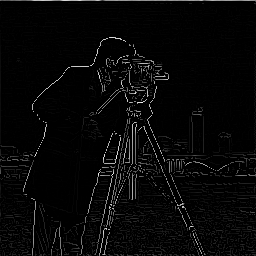
\includegraphics[scale = 0.5]{TpIFT6150-2-suppression.png}
    \caption{Normes des gradient post-supression}
\end{figure}
\section*{Description du but du seuillage pas hystérisis dans le filtre de Canny}
Comme on l'a mentionné brièvement dans la section* précédente, l'objectif du seuillage par hystérisis est d'éliminer les gradients qui ne se
retrouvent pas dans une certaines zones. Cette zone est délimiter par les variables $\tau_L$ et $\tau_H$. L'objectif de cette algorithme est relativement 
similaire à un algorithme de type \textit{flood fill}. Cependant, plutôt que de remplir une zone délimiter par un contour, on rempli les contours selon
les valeurs de $\tau_H$ et $\tau_L$. On a choisit d'implémenter une méthode récursive et itérative. La méthode récursive est assez simple. Elle itère sur tous
les pixels d'une image noire de même taille que l'image initiale (après la supression des non-maximums) et si le gradient de ce pixel est supérieur à notre borne
supérieure, on commence la procédure récursive. Cette procédure va ensuite vérifier si ce pixel est un contour (pixel blanc) ou pas (pixel noir) et si
la norme du gardient du pixel se trouve par-dessus la borne inférieure. Si c'est le cas, on colorie ce pixel en blanc et on obtient l'orientation 
de ce pixel et on applique la même procédure récursive à ses deux voisins les plus proches.
\begin{lstlisting}[language=C]
void follow(float** sups, int x, int y, int** orient, float** result, int width, int height, float tauL) {
    // If higher than lower bound and not a contour, then it becomes one

    if(sups[y][x] > tauL && result[y][x] == 0.f) {
        result[y][x] = 255.f;
        for(int i = 0; i < 4; i++) {
            int dir = orient[y][x];
            switch (dir) {
            case 0:
                if(x - 1 >= 0) {
                    follow(sups, x - 1, y, orient, result, width, height, tauL);
                }
                else if(x + 1 < width) {
                    follow(sups, x + 1, y, orient, result, width, height, tauL);
                }
            case 45:
                if(x + 1 < width && y - 1 >= 0) {
                    follow(sups, x + 1, y - 1, orient, result, width, height, tauL);
                }
                else if(x - 1 >= 0 && y + 1 < height) {
                    follow(sups, x - 1, y + 1, orient, result, width, height, tauL);
                }
            case 90:
                if(y - 1 >= 0) {
                    follow(sups, x, y - 1, orient, result, width, height, tauL);
                }
                else if(y + 1 < height) {
                    follow(sups, x, y + 1, orient, result, width, height, tauL);
                }
            case 135:
                if(x - 1 >= 0 && y - 1 >= 0) {
                    follow(sups, x - 1, y - 1, orient, result, width, height, tauL);
                }
                else if(x + 1 < width && y + 1 < height) {
                    follow(sups, x + 1, y + 1, orient, result, width, height, tauL);
                }
            }
        }
    }
}

void recursiveHysteresis(float** result, float** sups, int** orient, int width, int height, float tauL, float tauH) {
    for(int y = 0; y < height; y++) {
        for(int x = 0; x < width; x++) {
            if(sups[y][x] > tauH) {
                follow(sups, x, y, orient, result, width, height, tauL);
            }
        }
    }
}
\end{lstlisting}
La méthode itérative utilise les principes d'une queue. On commence par touvé les pixels avec une norme de gradient supérieure $\tau_H$. Ensuite, on itère
sur cette liste en ajoutant les voisins de ce pixel et on colorie les pixels en blanc si leur norme est supérieure à $\tau_L$ et en noir sinon.
\begin{lstlisting}[language=C]
void queueHysteresis(float** result, float** sups, int** direction, int width, int height, float tauL, float tauH) {
    int maxq = height * width;
    int *qY = (int*)malloc(sizeof(int)*maxq);
    int *qX = (int*)malloc(sizeof(int)*maxq);
    int head = 0, tail = 0;

    for (int i = 0; i < height; ++i) {
        for (int j = 0; j < width; ++j) {
            if (sups[i][j] > tauH) {
                result[i][j] = 255.0f;
                qY[tail] = i; qX[tail] = j; ++tail;
            }
        }
    }

    while (head < tail) {
        int y = qY[head], x = qX[head]; ++head;
        for (int dy8 = -1; dy8 <= 1; ++dy8) {
            for (int dx8 = -1; dx8 <= 1; ++dx8) {
                if (dy8 == 0 && dx8 == 0) continue;
                int ny = y + dy8, nx = x + dx8;
                if (ny < 0 || ny >= height || nx < 0 || nx >= width) continue;

                if (result[ny][nx] == 0.0f && sups[ny][nx] >= tauL) {
                    result[ny][nx] = 255.0f;
                    qY[tail] = ny; qX[tail] = nx; ++tail;
                }
            }
        }
    }  
}
\end{lstlisting}
Voici le résultat de chacune des méthodes:
\begin{figure}[H]
    \centering
    \begin{subfigure}[b]{0.45\linewidth}
        \centering
        
\includegraphics[scale = 0.5]{TpIFT6150-2-canny_queue.png}
        \caption{Méthode queue}
    \end{subfigure}
    \begin{subfigure}[b]{0.45\linewidth}
        \centering
        
\includegraphics[scale = 0.5]{TpIFT6150-2-canny_recursive.png}
        \caption{Méthode récursive}
    \end{subfigure}
    \caption{$\sigma = 1$, $\tau_H = 66$ et $\tau_L = 33$}
\end{figure}
\section*{Discussion et conclusion}
Lors de ce devoir, on a dû implémenter plusieurs façons de traiter la même image. Ce que l'on remarque est que les résultats de la méthode normale
et la méthode par histogramme de l'algorithme de Canny nous donne des résultats très similaires (si $p_H = 0.9$ et $\tau_H = 66$ et $\tau_L = 33$). 
Cependant, la méthode par histogramme nous donne un meilleur contrôle sur la quantité de gradients que l'on veut considérer comme un contour
(ce qui est logique considérant que c'est le but de cette méthode). Comme on s'y attendait, plus l'écart type $\sigma$ su filtre gaussien était élevé,
plus le \textbf{blurring} de l'image allait être remarquable. Bien évidemment, plus le \textbf{blurring} était élevé, moins l'isolation des contours étaient 
précises.
\begin{figure}[H]
    \begin{subfigure}[b]{0.45\linewidth}
        \centering
        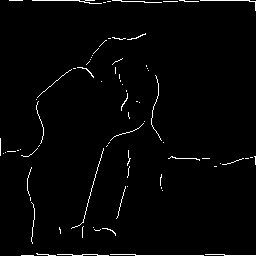
\includegraphics[scale = 0.5]{TpIFT6150-2-canny_10.png}
        \caption{$\sigma = 10$}
    \end{subfigure}
    \begin{subfigure}[b]{0.45\linewidth}
        \centering
        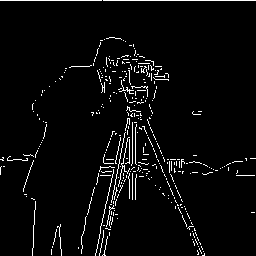
\includegraphics[scale = 0.5]{TpIFT6150-2-canny_09.png}
        \caption{$\sigma = 1$}
    \end{subfigure}
\end{figure}
Comme on a pus le voir aux figures 3, 4 et 5, on voit que la valeur de $p_H$ va avoir un effet assez prononcé sur le résultat final.
Si $p_H$ est faible, on va voir beaucoup plus de contours que si $p_H$ se rapproche de 1. En effet, si $p_H$ est faible, alors $\tau_H$ le sera aussi,
ce qui veut dire que l'on conserve plus de pixels lorsque l'on reconstruit les contours lors de l'hystérisis. On voit aussi que la méthode itérative et 
récursive donnent essentiellement les mêmes résultats. Voici ce que l'on obtient lorsque l'on applique la méthode normale et par histogramme sur l'image
mona.pgm.
\begin{figure}[H]
    \centering
    \begin{subfigure}[b]{0.45\linewidth}
        \centering
        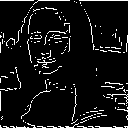
\includegraphics[scale = 1]{TpIFT6150-2-mona_norm.png}
        \caption{Méthode normale}
    \end{subfigure}
    \begin{subfigure}[b]{0.45\linewidth}
        \centering
        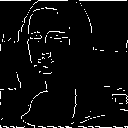
\includegraphics[scale = 1]{TpIFT6150-2-mona_noBin.png}
        \caption{Méthode par histogramme sans \textbf{bins}}
    \end{subfigure}
    \vspace{1em}
    \begin{subfigure}[b]{0.45\linewidth}
        \centering
        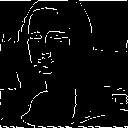
\includegraphics[scale = 1]{TpIFT6150-2-mona_binAVG.png}
        \caption{Méthode par histogramme avec \textbf{bins} moyenne}
    \end{subfigure}
    \begin{subfigure}[b]{0.45\linewidth}
        \centering
        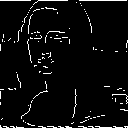
\includegraphics[scale = 1]{TpIFT6150-2-mona_binMED.png}
        \caption{Méthode par histogramme avec \textbf{bins} médiane}
    \end{subfigure}
    \caption{Mona.pgm avec $\sigma = 1$, $\tau_H = 66$, $\tau_L = 33$ et $p_H = 0.9$}
\end{figure}
\end{document}